\documentclass[]{book}
\usepackage{lmodern}
\usepackage{amssymb,amsmath}
\usepackage{ifxetex,ifluatex}
\usepackage{fixltx2e} % provides \textsubscript
\ifnum 0\ifxetex 1\fi\ifluatex 1\fi=0 % if pdftex
  \usepackage[T1]{fontenc}
  \usepackage[utf8]{inputenc}
\else % if luatex or xelatex
  \ifxetex
    \usepackage{mathspec}
  \else
    \usepackage{fontspec}
  \fi
  \defaultfontfeatures{Ligatures=TeX,Scale=MatchLowercase}
\fi
% use upquote if available, for straight quotes in verbatim environments
\IfFileExists{upquote.sty}{\usepackage{upquote}}{}
% use microtype if available
\IfFileExists{microtype.sty}{%
\usepackage{microtype}
\UseMicrotypeSet[protrusion]{basicmath} % disable protrusion for tt fonts
}{}
\usepackage[margin=1in]{geometry}
\usepackage{hyperref}
\hypersetup{unicode=true,
            pdftitle={Ciencia de Datos y Políticas Públicas},
            pdfauthor={Antonio Vazquez Brust},
            pdfborder={0 0 0},
            breaklinks=true}
\urlstyle{same}  % don't use monospace font for urls
\usepackage{natbib}
\bibliographystyle{apalike}
\usepackage{color}
\usepackage{fancyvrb}
\newcommand{\VerbBar}{|}
\newcommand{\VERB}{\Verb[commandchars=\\\{\}]}
\DefineVerbatimEnvironment{Highlighting}{Verbatim}{commandchars=\\\{\}}
% Add ',fontsize=\small' for more characters per line
\usepackage{framed}
\definecolor{shadecolor}{RGB}{248,248,248}
\newenvironment{Shaded}{\begin{snugshade}}{\end{snugshade}}
\newcommand{\KeywordTok}[1]{\textcolor[rgb]{0.13,0.29,0.53}{\textbf{#1}}}
\newcommand{\DataTypeTok}[1]{\textcolor[rgb]{0.13,0.29,0.53}{#1}}
\newcommand{\DecValTok}[1]{\textcolor[rgb]{0.00,0.00,0.81}{#1}}
\newcommand{\BaseNTok}[1]{\textcolor[rgb]{0.00,0.00,0.81}{#1}}
\newcommand{\FloatTok}[1]{\textcolor[rgb]{0.00,0.00,0.81}{#1}}
\newcommand{\ConstantTok}[1]{\textcolor[rgb]{0.00,0.00,0.00}{#1}}
\newcommand{\CharTok}[1]{\textcolor[rgb]{0.31,0.60,0.02}{#1}}
\newcommand{\SpecialCharTok}[1]{\textcolor[rgb]{0.00,0.00,0.00}{#1}}
\newcommand{\StringTok}[1]{\textcolor[rgb]{0.31,0.60,0.02}{#1}}
\newcommand{\VerbatimStringTok}[1]{\textcolor[rgb]{0.31,0.60,0.02}{#1}}
\newcommand{\SpecialStringTok}[1]{\textcolor[rgb]{0.31,0.60,0.02}{#1}}
\newcommand{\ImportTok}[1]{#1}
\newcommand{\CommentTok}[1]{\textcolor[rgb]{0.56,0.35,0.01}{\textit{#1}}}
\newcommand{\DocumentationTok}[1]{\textcolor[rgb]{0.56,0.35,0.01}{\textbf{\textit{#1}}}}
\newcommand{\AnnotationTok}[1]{\textcolor[rgb]{0.56,0.35,0.01}{\textbf{\textit{#1}}}}
\newcommand{\CommentVarTok}[1]{\textcolor[rgb]{0.56,0.35,0.01}{\textbf{\textit{#1}}}}
\newcommand{\OtherTok}[1]{\textcolor[rgb]{0.56,0.35,0.01}{#1}}
\newcommand{\FunctionTok}[1]{\textcolor[rgb]{0.00,0.00,0.00}{#1}}
\newcommand{\VariableTok}[1]{\textcolor[rgb]{0.00,0.00,0.00}{#1}}
\newcommand{\ControlFlowTok}[1]{\textcolor[rgb]{0.13,0.29,0.53}{\textbf{#1}}}
\newcommand{\OperatorTok}[1]{\textcolor[rgb]{0.81,0.36,0.00}{\textbf{#1}}}
\newcommand{\BuiltInTok}[1]{#1}
\newcommand{\ExtensionTok}[1]{#1}
\newcommand{\PreprocessorTok}[1]{\textcolor[rgb]{0.56,0.35,0.01}{\textit{#1}}}
\newcommand{\AttributeTok}[1]{\textcolor[rgb]{0.77,0.63,0.00}{#1}}
\newcommand{\RegionMarkerTok}[1]{#1}
\newcommand{\InformationTok}[1]{\textcolor[rgb]{0.56,0.35,0.01}{\textbf{\textit{#1}}}}
\newcommand{\WarningTok}[1]{\textcolor[rgb]{0.56,0.35,0.01}{\textbf{\textit{#1}}}}
\newcommand{\AlertTok}[1]{\textcolor[rgb]{0.94,0.16,0.16}{#1}}
\newcommand{\ErrorTok}[1]{\textcolor[rgb]{0.64,0.00,0.00}{\textbf{#1}}}
\newcommand{\NormalTok}[1]{#1}
\usepackage{longtable,booktabs}
\usepackage{graphicx,grffile}
\makeatletter
\def\maxwidth{\ifdim\Gin@nat@width>\linewidth\linewidth\else\Gin@nat@width\fi}
\def\maxheight{\ifdim\Gin@nat@height>\textheight\textheight\else\Gin@nat@height\fi}
\makeatother
% Scale images if necessary, so that they will not overflow the page
% margins by default, and it is still possible to overwrite the defaults
% using explicit options in \includegraphics[width, height, ...]{}
\setkeys{Gin}{width=\maxwidth,height=\maxheight,keepaspectratio}
\IfFileExists{parskip.sty}{%
\usepackage{parskip}
}{% else
\setlength{\parindent}{0pt}
\setlength{\parskip}{6pt plus 2pt minus 1pt}
}
\setlength{\emergencystretch}{3em}  % prevent overfull lines
\providecommand{\tightlist}{%
  \setlength{\itemsep}{0pt}\setlength{\parskip}{0pt}}
\setcounter{secnumdepth}{5}
% Redefines (sub)paragraphs to behave more like sections
\ifx\paragraph\undefined\else
\let\oldparagraph\paragraph
\renewcommand{\paragraph}[1]{\oldparagraph{#1}\mbox{}}
\fi
\ifx\subparagraph\undefined\else
\let\oldsubparagraph\subparagraph
\renewcommand{\subparagraph}[1]{\oldsubparagraph{#1}\mbox{}}
\fi

%%% Use protect on footnotes to avoid problems with footnotes in titles
\let\rmarkdownfootnote\footnote%
\def\footnote{\protect\rmarkdownfootnote}

%%% Change title format to be more compact
\usepackage{titling}

% Create subtitle command for use in maketitle
\newcommand{\subtitle}[1]{
  \posttitle{
    \begin{center}\large#1\end{center}
    }
}

\setlength{\droptitle}{-2em}

  \title{Ciencia de Datos y Políticas Públicas}
    \pretitle{\vspace{\droptitle}\centering\huge}
  \posttitle{\par}
  \subtitle{Una introducción a la exploración, análisis y visualización de datos}
  \author{Antonio Vazquez Brust}
    \preauthor{\centering\large\emph}
  \postauthor{\par}
      \predate{\centering\large\emph}
  \postdate{\par}
    \date{2019-04-04}

\usepackage{booktabs}

\begin{document}
\maketitle

{
\setcounter{tocdepth}{1}
\tableofcontents
}
\chapter*{}\label{section}
\addcontentsline{toc}{chapter}{}

Placeholder

\section*{Antes de empezar}\label{antes-de-empezar}
\addcontentsline{toc}{section}{Antes de empezar}

\chapter{¿Qué es la ciencia de datos?}\label{que-es-la-ciencia-de-datos}

Placeholder

\section{¿Qué significa hacer ciencia de
datos?}\label{que-significa-hacer-ciencia-de-datos}

\chapter{Una presentación a toda marcha de
R}\label{una-presentacion-a-toda-marcha-de-r}

\texttt{R} es un lenguaje de programación especializado en análisis y
visualización de datos. Es un producto de código abierto, lo cual
significa que cualquier persona puede usarlo y modificarlo sin pagar
licencias ni costos de adquisición de ningún tipo.

Expertos de todo el mundo colaboran en forma activa con el proyecto, no
sólo desarrollando el lenguaje en sí (llamado ``R base''), sino también
extendiéndolo con nuevas habilidades que pueden ser incorporadas por los
usuarios finales en forma de ``paquetes'' instalables.

La calidad del lenguaje en sí, de los paquetes instalables que le
agregan un sinfín de funciones (desde algoritmos de inteligencia
artificial hasta mapas interactivos) y de la comunidad de usuarios que
comparte información en foros y blogs, ha hecho de R uno de los
lenguajes de programación más populares del mundo. En el campo del
análisis de datos, es la herramienta por excelencia en muchas
universidades, empresas de tecnología, y redacciones de periodismo de
datos.

\section{Nuestro primer proyecto en
R}\label{nuestro-primer-proyecto-en-r}

A continuación reproduciremos un ejercicio paso a paso, para ilustrar la
potencia de una herramienta de análisis como R. Que nadie se preocupe si
algunas de las operaciones parecen no tener sentido, o resultan
arbitrarias. ¡Es normal! Nadie aprende un lenguaje en 10 minutos, sea R
o esperanto. La idea es tener exposición temprana a un caso de uso
interesante, usando datos reales. Y que nos sirva como motivación para
practicar luego ejercicios básicos que son muy necesarios pero, a veces,
no tan emocionantes.

\subsection{Crear un proyecto en
RStudio}\label{crear-un-proyecto-en-rstudio}

El primer paso es ejecutar RStudio, que ya deberíamos tener disponible
en nuestro sistema.

Una vez abierta la interfaz gráfica, creamos un proyecto nuevo,
cliqueando en
\texttt{File\ -\textgreater{}\ New\ Project...\ -\textgreater{}\ New\ Directory\ -\textgreater{}\ \ New\ Project}.
En la ventana que surge, elegir un nombre para el proyecto (por ejemplo,
``Practicando R'') y finalizar la operación cliqueando en
\texttt{Create\ project}.

Utilizar proyectos nos permite continuar otro día desde donde dejamos la
tarea al terminar una sesión. Es sólo cuestión de recuperar el proyecto
deseado la próxima vez que abrimos RStudio, cliqueando en
\texttt{File\ -\textgreater{}\ Recent\ Projects\ -\textgreater{}\ "nombre\ de\ mi\ proyecto"}.

Por ahora, sigamos trabajando. Vamos a crear un ``script''. Un script,
como su nombre en inglés lo indica, es un guión; una serie de pasos que
escribimos para que nuestra computadora ejecute en secuencia. Cliqueamos
en
\texttt{File\ -\textgreater{}\ New\ File\ -\textgreater{}\ R\ Script}.
De inmediato se abre una ventana con un editor de texto. ¡Ahora empieza
la acción!

\subsection{Escribiendo un script}\label{escribiendo-un-script}

Aprovechemos para dar un nombre a los áreas que vemos en RStudio:

\begin{figure}
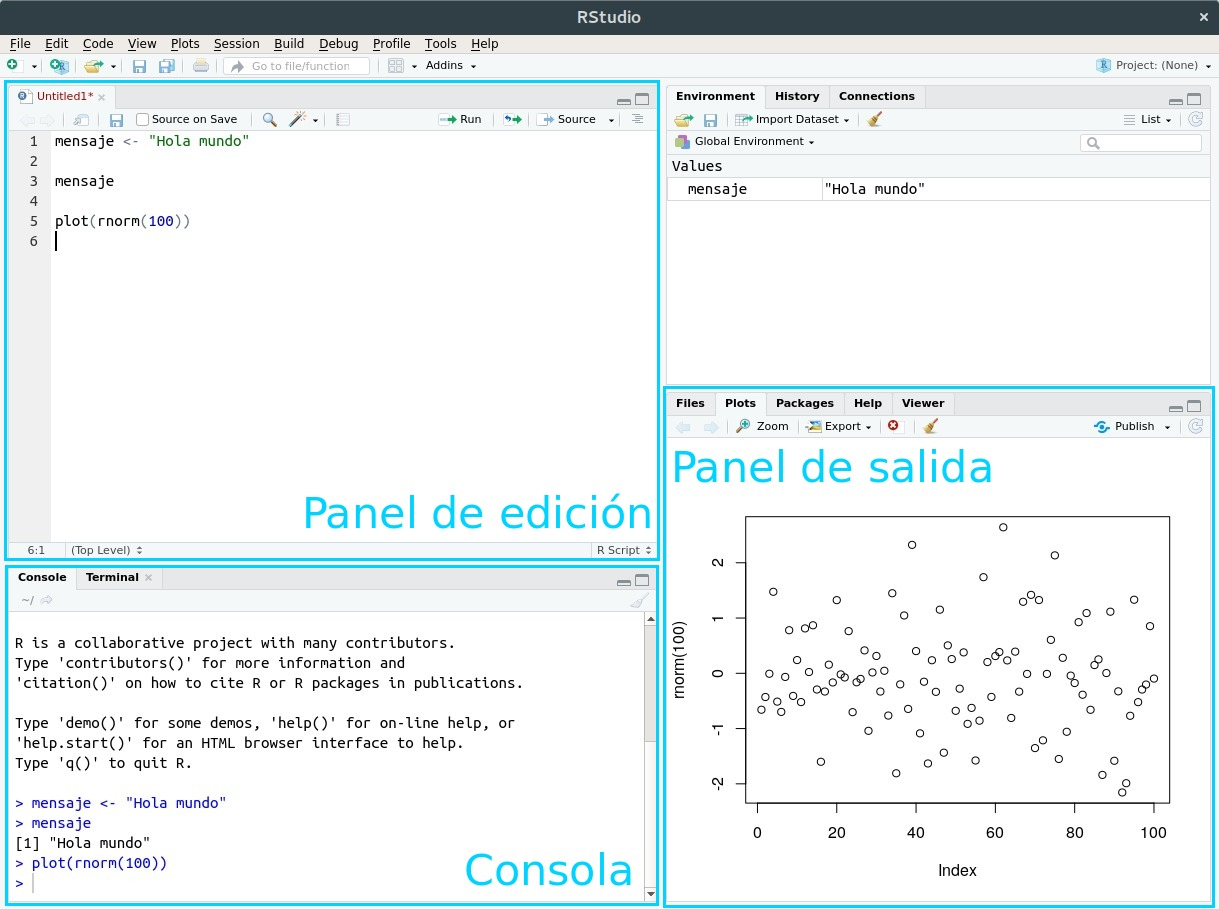
\includegraphics[width=1\linewidth]{imagenes/Interfaz_RStudio} \caption{La interfaz de RStudio}\label{fig:unnamed-chunk-1}
\end{figure}

Vamos a escribir nuestro código (las instrucciones que \texttt{R}
entiende) en el panel de edición. Los resultados van a aparecer en la
consola (cuando se trate de texto) o en el panel de salida (cuando
produzcamos gráficos)

Por ejemplo, podemos escribir el panel de edición la instrucción para
mostrar el resultado de una operación matemático:

\begin{Shaded}
\begin{Highlighting}[]
\KeywordTok{sqrt}\NormalTok{(}\DecValTok{144}\NormalTok{)}
\end{Highlighting}
\end{Shaded}

\texttt{sqrt()} es una \emph{función}. En el mundo de la programación,
las funciones son secuencias de código ya listas para usar, que realizan
tareas útiles. Por ejemplo, mostrar algo en pantalla. En nuestro caso,
completamos la función con algo más: un \emph{parámetro}, pues así se le
llama a los valores que una función espera de parte del usuario para
saber que hacer. La función print espera que le demos un número para el
cual calcular su raíz cuadrada (\emph{square root} en inglés), y eso
hicimos: le pasamos cómo parámetro \texttt{144}, un número. Los
parámetros siempre se escriben entre paréntesis, a continuación del
nombre de la función.

Ahora vamos a aprender la combinación de teclas más importante al usar
RStudio: \texttt{Ctrl} + \texttt{Enter}. Presionar \texttt{Ctrl} +
\texttt{Enter} al terminar de escribir una instrucción hace que RStudio
la ejecute de inmediato, y espere en la siguiente instrucción, si la
hubiera.

Cambien podemos buscar una línea que deseemos ejecutar, posicionando el
cursor de texto (que luce como una barra vertical que titila, en el
panel de edición) sobre ella. Si a continuación pulsamos \texttt{Ctrl} +
\texttt{Enter}, la línea será ejecutada y el cursor se moverá sólo hasta
la siguiente línea, listo para repetir el proceso.

La modalidad de ejecución línea por línea es muy útil para lo que se
llama ``análisis interactivo''. Uno ejecuta un comando, observa el
resultado, y en base a eso decide su próxima acción: cambiar parámetros
e intentarlo de nuevo, dar por buenos los resultados y usarlos para una
tarea subsiguiente\ldots{} etc.

Por ejemplo, si escribimos las siguientes líneas:

\begin{Shaded}
\begin{Highlighting}[]
\KeywordTok{sqrt}\NormalTok{(}\DecValTok{144}\NormalTok{)}

\NormalTok{mensaje <-}\StringTok{ "Hola mundo"}

\NormalTok{mensaje}
\end{Highlighting}
\end{Shaded}

\ldots{}y posicionamos el cursor en cualquier posición de la primera
línea, para luego pulsar \texttt{Ctrl} + \texttt{Enter} tres veces,
veremos que las instrucciones son ejecutadas línea a línea.

\begin{Shaded}
\begin{Highlighting}[]
\KeywordTok{sqrt}\NormalTok{(}\DecValTok{144}\NormalTok{)}
\end{Highlighting}
\end{Shaded}

\begin{verbatim}
## [1] 12
\end{verbatim}

\begin{Shaded}
\begin{Highlighting}[]
\NormalTok{mensaje <-}\StringTok{ "Hola mundo"}
\end{Highlighting}
\end{Shaded}

\begin{Shaded}
\begin{Highlighting}[]
\NormalTok{mensaje}
\end{Highlighting}
\end{Shaded}

\begin{verbatim}
## [1] "Hola mundo"
\end{verbatim}

Dos de ellas (la primera y la última) mostraron una salida en pantalla,
y la del medio, no. Esto es porque algunas funciones entregan algo como
resultado algo -un número, un texto, un gráfico, u otros tipos de salida
que ya veremos- mientras que otras hacen su tarea silenciosamente sin
expresar nada. En este caso, la función silenciosa fue la de asignación:
\texttt{mensaje\ \textless{}-\ "Hola\ mundo"} es una instrucción que le
pide a R que cree una variable llamada ``mensaje'' (o que la encuentre
si ya existe) y que le asigne como valor el texto ``Hola mundo''. ¿Cómo
sabemos que la instrucción se llevó a cabo, a pesar de no producir una
salida? En general, es un tema de confianza. Si una instrucción no
genera un mensaje de error, si es silenciosa, se asume que pudo cumplir
su cometido. En este caso, además lo hemos verificado. La línea final,
\texttt{mensaje} pide a R que busque la variable, y muestre en pantalla
su contenido (esa es una característica muy práctica del lenguaje: para
saber el contenido de una variable, basta con escribirla y ejecutar la
línea). Y al hacerlo, comprobamos que la variable contiene precisamente
lo que hemos tipeado.

De paso, hay que mencionar que la creación y manipulación de variables
es un concepto clave en programación. Trabajar con variables nos permite
almacenar valores para usarlos después, además de hacer nuestro código
más fácil de leer y compartir con otros, en especial cuando usamos
nombre de variable auto-explicativos. Como ejemplo de ésto ultimo
comparemos

\begin{Shaded}
\begin{Highlighting}[]
\NormalTok{x <-}\StringTok{ }\DecValTok{8} \OperatorTok{*}\StringTok{ }\DecValTok{6}
\NormalTok{x}
\end{Highlighting}
\end{Shaded}

\begin{verbatim}
## [1] 48
\end{verbatim}

\ldots{} con

\begin{Shaded}
\begin{Highlighting}[]
\NormalTok{ancho_habitacion_m <-}\StringTok{ }\DecValTok{8}
\NormalTok{profundiad_habitacion_m <-}\StringTok{ }\DecValTok{6}
\NormalTok{superficie_habitacion_m2 <-}\StringTok{ }\NormalTok{ancho_habitacion_m }\OperatorTok{*}\StringTok{ }\NormalTok{profundiad_habitacion_m}

\NormalTok{superficie_habitacion_m2}
\end{Highlighting}
\end{Shaded}

\begin{verbatim}
## [1] 48
\end{verbatim}

En su resultado ambas expresiones son iguales, dado que producen lo
mismo. Pero la segunda esta escrita de una forma mucho más clara para un
ser humano, que hace más fácil interpretar su lógica\ldots{} ¡está
calculando la superficie en metros cuadrados de una habitación!. Es muy
importante escribir nuestro código de la forma más explícita posible,
aunque requiera tipear un poco más. Con ello, le hacemos la vida más
fácil a otras personas que interpreten nuestros programas. Y también a
nosotros mismos en el futuro, cuando debamos lidiar con un programa que
escribimos tiempo atrás y del que a duras penas recordamos su lógica.

\section{Un ejemplo de análisis paso a
paso}\label{un-ejemplo-de-analisis-paso-a-paso}

Imaginemos por un momento que trabajamos en un área del Gobierno de la
Ciudad encargada de analizar los reclamos y solicitudes que realizan los
vecinos. Para abordar el tema, algunas preguntas que de inmediato vienen
a la mente son ¿Qué tipo de solicitudes hacen los ciudadanos, en qué
cantidad, y en dónde?

Disponiendo de los datos necesarios, podemos usar \texttt{R} para
encontrar las respuestas.

Vamos a cargar datos provenientes de los registros del Sistema Único de
Atención Ciudadana (o \href{https://suaci.buenosaires.gob.ar}{SUACI}),
la plataforma del Gobierno de la Ciudad que administra los contactos
iniciados por ciudadanos. En el portal de datos abiertos de la Ciudad se
publica
\href{https://data.buenosaires.gob.ar/dataset/sistema-unico-atencion-ciudadana}{cada
uno de los contactos recibidos por SUACI año a año}. El tipo de archivo
con el que se publican es ``.csv'' (o ``comma separated values'') un
formato muy popular en el mundo de la ciencia de datos, ya que es muy
fácil de manipular y compartir entre sistemas. Es posible abrir un
archivo .csv hasta con el
\href{https://es.wikipedia.org/wiki/Bloc_de_notas}{humilde block de
notas}. Al igual que los archivos .xls, los .csv se utilizan para
guardar información tabular: un rectángulo con filas y columnas. R
incluye una función que lee archivos .csv, que se llama
\texttt{read.csv}. La usamos así:

\begin{Shaded}
\begin{Highlighting}[]
\NormalTok{suaci2018 <-}\StringTok{ }\KeywordTok{read.csv}\NormalTok{(}\StringTok{'https://bitsandbricks.github.io/data/gcba_suaci_2018.csv'}\NormalTok{)}
\end{Highlighting}
\end{Shaded}

Obsérvese que los datos están alojados en un servidor de internet
(accesibles vía \textbf{\url{https://bitsandbricks}\ldots{}}). Eso no es
problema para la función read.csv, que con la misma soltura lee archivos
guardados en nuestra PC o publicados en un sitio web. Para ver el
contenido de la variable donde guardamos el resultado de leer la data,
\texttt{suaci2018}, sólo hace falta escribir su nombre:

\begin{Shaded}
\begin{Highlighting}[]
\NormalTok{suaci2018}
\end{Highlighting}
\end{Shaded}

\begin{verbatim}
##               BARRIO CONTACTOS
## 1          AGRONOMIA      7378
## 2            ALMAGRO     31420
## 3          BALVANERA     28616
## 4           BARRACAS     23106
## 5           BELGRANO     46936
## 6               BOCA     11495
## 7              BOEDO     12926
## 8          CABALLITO     50301
## 9          CHACARITA     11076
## 10           COGHLAN      8920
## 11        COLEGIALES     18637
## 12      CONSTITUCION      7569
## 13            FLORES     38462
## 14          FLORESTA     13589
## 15           LINIERS     17606
## 16         MATADEROS     19771
## 17         MONSERRAT     10716
## 18      MONTE CASTRO     15459
## 19     NUEVA POMPEYA     11762
## 20             NUÑEZ     26556
## 21           PALERMO     75068
## 22 PARQUE AVELLANEDA     14914
## 23  PARQUE CHACABUCO     16560
## 24       PARQUE CHAS      8948
## 25  PARQUE PATRICIOS     13559
## 26          PATERNAL      7255
## 27     PUERTO MADERO      1939
## 28          RECOLETA     30339
## 29            RETIRO     10646
## 30          SAAVEDRA     18232
## 31     SAN CRISTOBAL     11050
## 32       SAN NICOLAS     12526
## 33         SAN TELMO      5281
## 34   VELEZ SARSFIELD     11586
## 35         VERSALLES      5835
## 36      VILLA CRESPO     25748
## 37  VILLA DEL PARQUE     25224
## 38      VILLA DEVOTO     34361
## 39 VILLA GRAL. MITRE     11417
## 40      VILLA LUGANO     24853
## 41        VILLA LURO     11485
## 42     VILLA ORTUZAR     11150
## 43  VILLA PUEYRREDON     18985
## 44        VILLA REAL      5496
## 45   VILLA RIACHUELO      5311
## 46  VILLA SANTA RITA     13265
## 47     VILLA SOLDATI      9811
## 48     VILLA URQUIZA     40146
\end{verbatim}

Vemos que la tabla tiene 48 filas (una por cada barrio de la ciudad) y 2
columnas (una con el nombre del barrio, y otra con la cantidad total de
contactos registrados en 2018).

En R, las tablas son llamadas \texttt{dataframes}. El dataframe es el
objeto por excelencia del análisis de datos. En concepto, es muy similar
a una tabla de excel; al fin y al cabo, ambos formatos guardan
información en celdas identificadas por fila y columna.

Algunas funciones útiles para explorar un dataframe que no conocemos son
\texttt{dim()}, que nos da las dimensiones del dataframe (cantidad de
filas y columnas), \texttt{names()} que nos dice como se llaman sus
columnas (que en general representan variables), y \texttt{head()} que
nos permite echar un vistazo rápido al contenido, mostrando sólo las
seis primeras filas (ésto es útil porque con frecuencia trabajamos con
dataframes que contienen miles o millones de filas, con lo que no tiene
sentido tratar de volcar todas en pantalla).

\begin{Shaded}
\begin{Highlighting}[]
\KeywordTok{dim}\NormalTok{(suaci2018)}
\end{Highlighting}
\end{Shaded}

\begin{verbatim}
## [1] 48  2
\end{verbatim}

\begin{Shaded}
\begin{Highlighting}[]
\KeywordTok{names}\NormalTok{(suaci2018)}
\end{Highlighting}
\end{Shaded}

\begin{verbatim}
## [1] "BARRIO"    "CONTACTOS"
\end{verbatim}

\begin{Shaded}
\begin{Highlighting}[]
\KeywordTok{head}\NormalTok{(suaci2018)}
\end{Highlighting}
\end{Shaded}

\begin{verbatim}
##      BARRIO CONTACTOS
## 1 AGRONOMIA      7378
## 2   ALMAGRO     31420
## 3 BALVANERA     28616
## 4  BARRACAS     23106
## 5  BELGRANO     46936
## 6      BOCA     11495
\end{verbatim}

\section{Visualización: la exploración gráfica de la
información}\label{visualizacion-la-exploracion-grafica-de-la-informacion}

Ahora es vamos a pisar el acelerador. Insisto: nadie debe preocuparse si
algunos conceptos parecen ser demasiado complejos. En las próximas
secciones practicaremos de forma gradual las técnicas que vamos a usar
ahora, y todo tendrá sentido -¡lo prometo!. Pero antes, seamos un
poquito irresponsables con el poder de R y empleemos un arsenal
sofisticado de herramientas para ver de que somos capaces.

En la introducción hablamos de los paquetes, conjuntos de programas que
extienden la funcionalidad de R. Vamos a cargar uno de los paquetes más
usados, \texttt{tidyverse}. Tidyverse incluye una gran cantidad de
funciones diseñadas por y para practicantes de la ciencia de datos.
Estas funciones comparten una filosofía y una sintaxis común, por lo que
al aprender una en cierto modo aprendemos a usar todas. El valor que
aportan es que, sin dudas, ayudan a realizar de manera más fácil las
tareas típicas de la ciencia de datos: importar, limpiar, comprender y
comunicar datos.

Si acabamos de instalar R y RStudio, el paquete aún no estará disponible
en nuestro sistema. Para instalarlo, usamos la función
\texttt{install.packages()} y le pasamos el nombre del paquete deseado,
``tidyverse'', entre comillas.

\begin{Shaded}
\begin{Highlighting}[]
\KeywordTok{install.packages}\NormalTok{(}\StringTok{"tidyverse"}\NormalTok{)}
\end{Highlighting}
\end{Shaded}

De aquí en más, podremos activar el conjunto de funciones que provee
\texttt{tidyverse} cada vez que queramos. Para eso, lo invocamos con la
función \texttt{library()}:

\begin{Shaded}
\begin{Highlighting}[]
\KeywordTok{library}\NormalTok{(tidyverse)}
\end{Highlighting}
\end{Shaded}

\begin{verbatim}
## -- Attaching packages -------------------------------------------------------------- tidyverse 1.2.1 --
\end{verbatim}

\begin{verbatim}
## v ggplot2 3.1.0       v purrr   0.3.0  
## v tibble  2.1.1       v dplyr   0.8.0.1
## v tidyr   0.8.2       v stringr 1.4.0  
## v readr   1.3.1       v forcats 0.2.0
\end{verbatim}

\begin{verbatim}
## -- Conflicts ----------------------------------------------------------------- tidyverse_conflicts() --
## x dplyr::filter() masks stats::filter()
## x dplyr::lag()    masks stats::lag()
\end{verbatim}

\ldots{} y listo para usar. La razón por la cual activamos tidyverse es
que en este momento nos vienen bien dos de sus funciones:
\texttt{mutate()} para modificar valores, y \texttt{ggplot()} para hacer
gráficos.

Bien, llega la hora presentar información en forma visual. Vamos a
llamar a la función \texttt{ggplot()}, una auténtica navaja suiza para
la visualización.

Por ejemplo, veamos cuantos contactos sumó cada barrio durante 2018:

\begin{Shaded}
\begin{Highlighting}[]
\KeywordTok{ggplot}\NormalTok{(suaci2018) }\OperatorTok{+}
\StringTok{    }\KeywordTok{geom_col}\NormalTok{(}\KeywordTok{aes}\NormalTok{(}\DataTypeTok{x =}\NormalTok{ BARRIO, }\DataTypeTok{y =}\NormalTok{ CONTACTOS)) }\OperatorTok{+}
\StringTok{    }\KeywordTok{coord_flip}\NormalTok{()}
\end{Highlighting}
\end{Shaded}

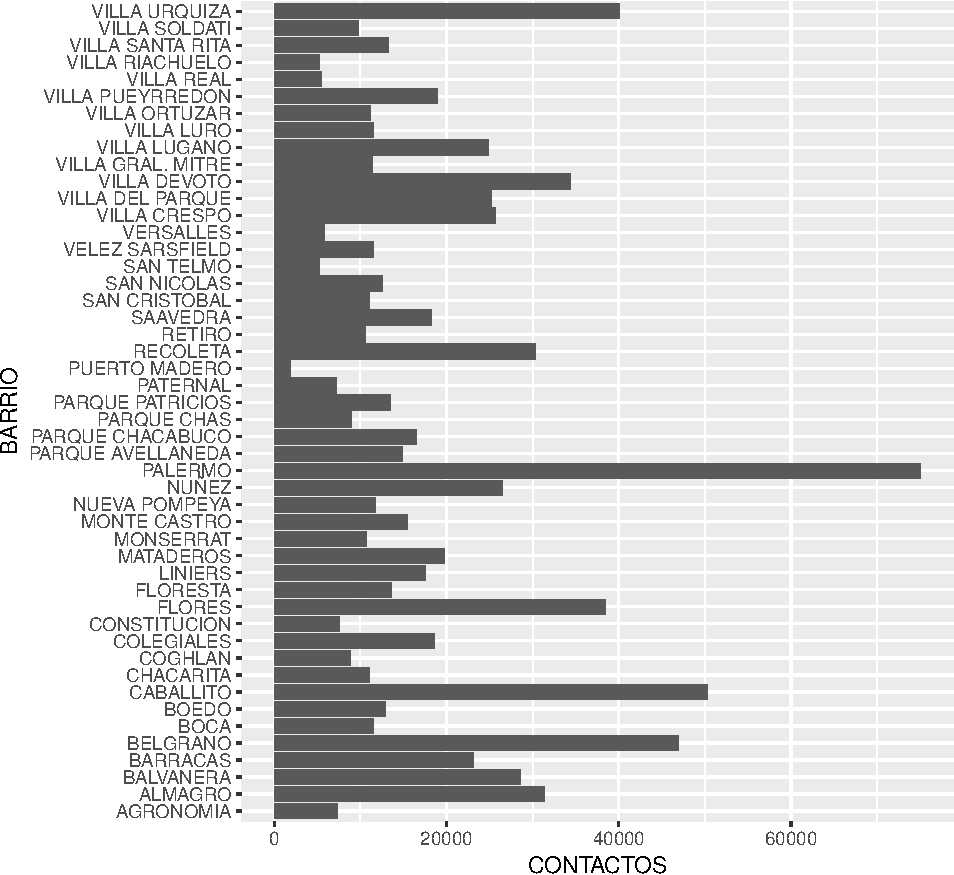
\includegraphics{ciencia_de_datos_politicas_publicas_files/figure-latex/unnamed-chunk-14-1.pdf}

Para realizar una visualización con ésta herramienta, siempre se
comienza con la función \texttt{ggplot()}, que crea un eje de
coordenadas sobre el cual se pueden agregar capas. El primer parámetro
que recibe \texttt{ggplot()} es el dataset que queremos usar para el
gráfico; en nuestro caso, \texttt{ggplot(suaci2018)}. Ejecutar sólo
\texttt{ggplot(suaci2018)} nos devuelve un gráfico vacío; la gracia está
en agregar una o más capas especificando cómo queremos mostrar los
datos. Estas capas se agregan con un signo \texttt{+}.

En nuestro ejemplo, \texttt{geom\_col()} crea columnas cuya posición en
el eje vertical depende de la variable ``BARRIO'', mientas que la
extensión (posición en el eje horizontal) depende del valor de la
variable ``CONTACTOS''. Existen muchas funciones del tipo ``geom\_XXX'',
que agregan distintas clases de capas al gráfico: geom\_point,
geom\_polygon, geom\_text y muchos, muchos más que iremos viendo más
adelante.

Cada función ``geom\_'' toma como parámetro un conjunto de definiciones
``estéticas'' que le indican una variable a graficar (``CANTIDAD'' en
nuestro caso), cómo representar los valores (por color, tamaño, etc) y
en dónde (posición en el eje x, posición en el eje y). Estos parámetros
van siempre dentro de una función auxiliar, \texttt{aes()}. En nuestro
ejemplo, ``aes(x = BARRIO, y = contactos)''. La última línea,
``coord\_flip()'', cambia la disposición de los ejes; en lugar de las x
en horizontal y las y en vertical, al revés. ¿Porqué es útil a veces
trastocar la posición de los ejes? Prueben correr la función sin agregar
esa línea,
\texttt{ggplot(suaci2018)\ +\ geom\_col(aes(x\ =\ BARRIO,\ y\ =\ CONTACTOS))},
y verán.

No se preocupen que iremos practicando el uso de ggplot, y su uso se
volverá familiar.

En cuanto al gráfico que hemos creado, podemos observar que entre las 48
barrios de la ciudad la cantidad de contactos en 2018 varió bastante. Si
escudriñamos las líneas podemos arriesgar que van de de un par de miles
en Puerto Madero a unos 75000 en Palermo. Lo que no nos muestra son
patrones espaciales: ¿Cómo es la distribución geográfica de las
solicitudes? ¿Los barrios con mayor demanda son los de una región de la
ciudad en particular? Para responde esas preguntas, necesitamos un mapa.

\subsection{Haciendo mapas}\label{haciendo-mapas}

Vamos a presentar un paquete más, el último para éste capítulo:
\texttt{sf}. Quizás algunos tengan experiencia con sistemas de
información geográfica (GIS por sus siglas en inglés), al estilo de
\href{https://qgis.org/en/site/}{QGIS} o
\href{https://www.arcgis.com/features/index.html}{ArcGIS}, que permiten
crear, manipular y combinar archivos con datos espaciales para producir
mapas que pueden ser simples o en extremo sofisticados. En R, el paquete
\texttt{sf} brinda herramientas que permiten realizar tares similares.

Nuestro objetivo es obtener un mapa de la ciudad de Buenos Aires con sus
comunas.

Primero, instalamos \texttt{sf} en caso de que aún no lo hayamos hecho.

\begin{Shaded}
\begin{Highlighting}[]
\KeywordTok{install.packages}\NormalTok{(}\StringTok{"sf"}\NormalTok{)}
\end{Highlighting}
\end{Shaded}

Vale la pena insistir: Sólo es necesario instalar los paquetes una vez.
De aquí en más, cada vez que querramos echar mano a las funciones
incluidas en \texttt{sf}, sólo necesitamos activarlo pues ya estará
listo en nuestro sistema. Pedimos a R que active el paquete así:

\begin{Shaded}
\begin{Highlighting}[]
\KeywordTok{library}\NormalTok{(sf)}
\end{Highlighting}
\end{Shaded}

\begin{verbatim}
## Linking to GEOS 3.6.2, GDAL 2.2.3, PROJ 4.9.3
\end{verbatim}

Luego, cargamos un archivo georeferenciado con las comunas de la Ciudad
Autónoma de Buenos Aires, disponible online en formato
\href{https://es.wikipedia.org/wiki/GeoJSON}{\emph{geojson}}, un
estándar de representación de datos geográficos que es fácil de usar:

\begin{Shaded}
\begin{Highlighting}[]
\NormalTok{barrios <-}\StringTok{ }\KeywordTok{st_read}\NormalTok{(}\StringTok{'https://bitsandbricks.github.io/data/CABA_barrios.geojson'}\NormalTok{)}
\end{Highlighting}
\end{Shaded}

\begin{verbatim}
## Reading layer `CABA_barrios' from data source `https://bitsandbricks.github.io/data/CABA_barrios.geojson' using driver `GeoJSON'
## Simple feature collection with 48 features and 4 fields
## geometry type:  POLYGON
## dimension:      XY
## bbox:           xmin: -58.53152 ymin: -34.70529 xmax: -58.33514 ymax: -34.52754
## epsg (SRID):    4326
## proj4string:    +proj=longlat +datum=WGS84 +no_defs
\end{verbatim}

Al igual que cuando usamos \texttt{read.csv()} para leer un archivo .csv
y cargarlo como un dataframe, el comando \texttt{st\_read()} hace lo
propio con archivos de información geográfica, conocidos en la jerga
como ``shapefiles''. El resultado también es un dataframe, por lo cual
podemos practicar el uso de las funciones que ya aprendimos, como dim(),
names() y head().

\begin{Shaded}
\begin{Highlighting}[]
\KeywordTok{dim}\NormalTok{(barrios)}
\end{Highlighting}
\end{Shaded}

\begin{verbatim}
## [1] 48  5
\end{verbatim}

\begin{Shaded}
\begin{Highlighting}[]
\KeywordTok{names}\NormalTok{(barrios)}
\end{Highlighting}
\end{Shaded}

\begin{verbatim}
## [1] "BARRIO"    "COMUNA"    "PERIMETRO" "AREA"      "geometry"
\end{verbatim}

\begin{Shaded}
\begin{Highlighting}[]
\KeywordTok{head}\NormalTok{(barrios)}
\end{Highlighting}
\end{Shaded}

\begin{verbatim}
## Simple feature collection with 6 features and 4 fields
## geometry type:  POLYGON
## dimension:      XY
## bbox:           xmin: -58.50617 ymin: -34.63064 xmax: -58.41192 ymax: -34.57829
## epsg (SRID):    4326
## proj4string:    +proj=longlat +datum=WGS84 +no_defs
##             BARRIO COMUNA PERIMETRO    AREA                       geometry
## 1        CHACARITA     15  7725.695 3118101 POLYGON ((-58.45282 -34.595...
## 2         PATERNAL     15  7087.513 2229829 POLYGON ((-58.46558 -34.596...
## 3     VILLA CRESPO     15  8132.699 3613584 POLYGON ((-58.42375 -34.597...
## 4 VILLA DEL PARQUE     11  7705.390 3399596 POLYGON ((-58.49461 -34.614...
## 5          ALMAGRO      5  8537.901 4050752 POLYGON ((-58.41287 -34.614...
## 6        CABALLITO      6 10990.964 6851029 POLYGON ((-58.43061 -34.607...
\end{verbatim}

Podemos ver que el dataframe contiene 48 filas y 5 columnas. Una fila
por barrio, y una columnas por cada variable disponible: ``BARRIO'',
``COMUNA'', ``PERIMETRO'', ``AREA'' y ``geometry''. Nuestro vistazo
mediante head() permite asumir que ``BARRIO'' contiene los nombres,
COMUNA indica la unidad administrativa, y PERIMETRO y AREA informan
sobre las dimensiones del polígono cubierto por cada barrio. La columna
``geometry'' aparece en todos los dataframes de tipo espacial, y es la
que contiene los datos con sus coordenadas geográficas.

Y hablando de coordenadas, generar un mapa a partir de un dataframe
espacial creado por sf es muy fácil con la ayuda de \texttt{ggplot()}:

\begin{Shaded}
\begin{Highlighting}[]
\KeywordTok{ggplot}\NormalTok{(barrios) }\OperatorTok{+}
\StringTok{    }\KeywordTok{geom_sf}\NormalTok{()}
\end{Highlighting}
\end{Shaded}

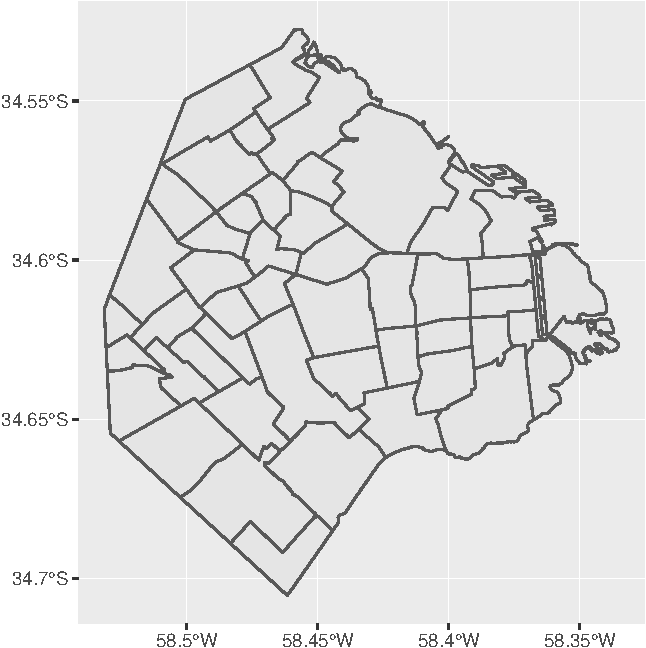
\includegraphics{ciencia_de_datos_politicas_publicas_files/figure-latex/unnamed-chunk-19-1.pdf}

Si queremos agregar una leyenda al mapa que identifique la comuna a la
que pertenece cada barrio, usamos:

\begin{Shaded}
\begin{Highlighting}[]
\KeywordTok{ggplot}\NormalTok{(barrios) }\OperatorTok{+}
\StringTok{    }\KeywordTok{geom_sf}\NormalTok{(}\KeywordTok{aes}\NormalTok{(}\DataTypeTok{fill =} \KeywordTok{factor}\NormalTok{(COMUNA)))}
\end{Highlighting}
\end{Shaded}

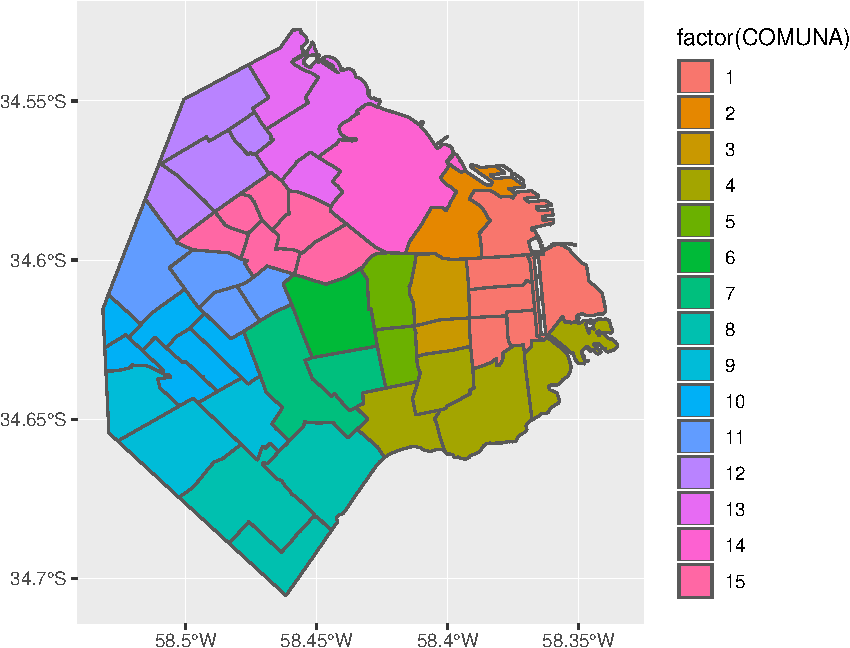
\includegraphics{ciencia_de_datos_politicas_publicas_files/figure-latex/unnamed-chunk-20-1.pdf}

Dentro de ``aes()'' usé el parámetro ``fill'' (relleno en inglés) para
pedirle a \texttt{ggplot()} que llene cada polígono con un color
distinto de acuerdo al campo ``COMUNA''. Lo mismo podríamos hacer para
ver la distribución de solicitudes registradas en SUACI, pintando los
barrios con una escala de colores que indique el nivel de solicitudes
que les corresponde. Pero antes de hacer eso, pensemos: es de esperarse
que los barrios más poblados representen un mayor número de solicitudes
que los más pequeños, ya que al fin y al cabo tienen más gente viviendo
dentro. Nos interesa la cantiad de contactos \emph{per cápita}, lo cuál
debería darnos una mejor idea acerca de las diferencias entre barrios en
lo que respecta a cuánta interacción hay entre vecinos y gobierno.

Sumemos pues datos de población.

\subsection{Agregando datos}\label{agregando-datos}

Cuando tenemos una identificador en común, \texttt{R} hace muy fácil
cruzar datos de fuentes distintas. Traigamos los datos de población en
cada barrio de la Ciudad de Buenos Aires, de acuerdo al censo nacional
de 2010:

\begin{Shaded}
\begin{Highlighting}[]
\NormalTok{poblacion <-}\StringTok{ }\KeywordTok{read.csv}\NormalTok{(}\StringTok{"https://bitsandbricks.github.io/data/caba_pob_barrios_2010.csv"}\NormalTok{)}
\end{Highlighting}
\end{Shaded}

Veamos el contenido del dataframe:

\begin{Shaded}
\begin{Highlighting}[]
\KeywordTok{head}\NormalTok{(poblacion)}
\end{Highlighting}
\end{Shaded}

\begin{verbatim}
##      BARRIO POBLACION
## 1 AGRONOMIA     13912
## 2   ALMAGRO    131699
## 3 BALVANERA    138926
## 4  BARRACAS     89452
## 5  BELGRANO    126267
## 6      BOCA     45113
\end{verbatim}

Bien, tenemos el nombre de cada barrio y su población. Como nuestro
dataframe de contactos a SUACI tiene una columna con el mismo nombre que
contiene las mismas categorías, sumarle la información de población es
tan fácil como:

\begin{Shaded}
\begin{Highlighting}[]
\NormalTok{suaci2018 <-}\StringTok{ }\KeywordTok{left_join}\NormalTok{(suaci2018, poblacion)}
\end{Highlighting}
\end{Shaded}

\begin{verbatim}
## Joining, by = "BARRIO"
\end{verbatim}

Más adelante aprenderemos más de las funciones de ``join'', que nos
permiten cruzar información. Por ahora sólo miremos el resultado:

\begin{Shaded}
\begin{Highlighting}[]
\KeywordTok{head}\NormalTok{(suaci2018)}
\end{Highlighting}
\end{Shaded}

\begin{verbatim}
##      BARRIO CONTACTOS POBLACION
## 1 AGRONOMIA      7378     13912
## 2   ALMAGRO     31420    131699
## 3 BALVANERA     28616    138926
## 4  BARRACAS     23106     89452
## 5  BELGRANO     46936    126267
## 6      BOCA     11495     45113
\end{verbatim}

Todo en orden. Ahora usemos una operación similar para sumar los datos
de SUACI y de pobación al dataframe con información espacial, el que nos
permite dibujar los barrios. Teniendo toda la información allí, podremos
visualizar el mapa que queremos.

\begin{Shaded}
\begin{Highlighting}[]
\NormalTok{barrios <-}\StringTok{ }\KeywordTok{left_join}\NormalTok{(barrios, suaci2018)}
\end{Highlighting}
\end{Shaded}

\begin{verbatim}
## Joining, by = "BARRIO"
\end{verbatim}

\section{El resultado final}\label{el-resultado-final}

Habrán notado que llegar hasta aquí tomó una buena cantidad de
operaciones. En contraste, lo que estamos a punto de hacer -generar un
mapa con los barrios de la ciudad que muestre la cantidad de solicitudes
de la ciudadanía per cápita- va a ser mucho más breve. Esa vendría a ser
la lección central de éste capítulo: la mayor parte del tiempo empleado
en la labor de la ciencia de datos se insume en la poco glamorosa tarea
de recopilar, limpiar y combinar los registros necesarios para el
análisis. Como consuelo, podemos pensar en que el esfuerzo necesario
para llegar a este punto nos ha dado un conocimiento de los datos (su
estructura, su contenido, atributos en común, etc) que no teníamos
antes.

Aprovechemos entonces nuestra data limpia y ordenada, para producir un
mapa que indique por color el grado en que los vecinos de cada barrio
interactúan con los canales de atención del gobierno de la Ciudad. Con
ggplot dibujaremos los barrios, y pintaremos su interior (``fill'') de
acuerdo a la cantidad de contactos, dividida por la población local. Por
último, definiremos la paleta de colores a usar en el \emph{fill},
eligiendo una escala llamada ``Spectral'', que va del azul al rojo y es
muy usada cuando se quiere resaltar la divergencia de una variable.

\begin{Shaded}
\begin{Highlighting}[]
\KeywordTok{ggplot}\NormalTok{(barrios) }\OperatorTok{+}
\StringTok{    }\KeywordTok{geom_sf}\NormalTok{(}\KeywordTok{aes}\NormalTok{(}\DataTypeTok{fill =}\NormalTok{ CONTACTOS }\OperatorTok{/}\StringTok{ }\NormalTok{POBLACION)) }\OperatorTok{+}
\StringTok{    }\KeywordTok{scale_fill_distiller}\NormalTok{(}\DataTypeTok{palette =} \StringTok{"Spectral"}\NormalTok{)}
\end{Highlighting}
\end{Shaded}

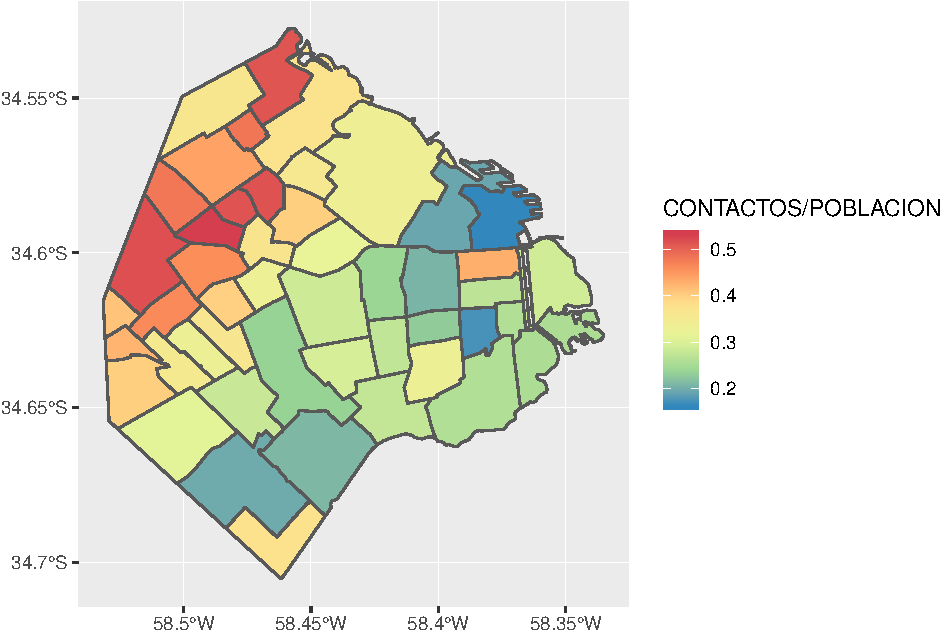
\includegraphics{ciencia_de_datos_politicas_publicas_files/figure-latex/unnamed-chunk-26-1.pdf}

¡Y hemos hallado un patrón! La zona caliente de contactos se asienta en
el sector noroeste de la Ciudad.

Por supuesto, con esto no puede darse por cerrado el tema; hay muchas
facetas que deberíamos analizar para comenzar a entender éste fenómeno
social o cualquier otro.

En los siguientes capítulos practicaremos varias técnicas que nos
permitirán profundizar nuestros análisis, en la nunca finalizada misión
de entender un poco más.

\chapter{Poniendo los datos en forma}\label{poniendo-los-datos-en-forma}

Placeholder

\section{Primeros pasos al examinar un conjunto de datos
nuevo}\label{primeros-pasos-al-examinar-un-conjunto-de-datos-nuevo}

\section{\texorpdfstring{Cruzando variables: la operación
\texttt{join}}{Cruzando variables: la operación join}}\label{cruzando-variables-la-operacion-join}

\section{Transformando los datos}\label{transformando-los-datos}

\subsection{\texorpdfstring{Seleccionar columnas con
\texttt{select()}}{Seleccionar columnas con select()}}\label{seleccionar-columnas-con-select}

\subsection{\texorpdfstring{Filtrar filas con
\texttt{filter()}}{Filtrar filas con filter()}}\label{filtrar-filas-con-filter}

\subsubsection{Comparaciones}\label{comparaciones}

\subsubsection{Operadores lógicos}\label{operadores-logicos}

\subsection{\texorpdfstring{Ordenar filas con
\texttt{arrange()}}{Ordenar filas con arrange()}}\label{ordenar-filas-con-arrange}

\subsubsection{Valores faltantes}\label{valores-faltantes}

\subsection{\texorpdfstring{Agregar nuevas variables con
\texttt{mutate()}}{Agregar nuevas variables con mutate()}}\label{agregar-nuevas-variables-con-mutate}

\subsection{\texorpdfstring{Extraer sumarios con
\texttt{summarise()}}{Extraer sumarios con summarise()}}\label{extraer-sumarios-con-summarise}

\subsection{\texorpdfstring{¡BONUS! El operador ``pipe'':
\texttt{\%\textgreater{}\%}}{¡BONUS! El operador pipe: \%\textgreater{}\%}}\label{bonus-el-operador-pipe}

\chapter{Visualización}\label{visualizacion}

Placeholder

\section{\texorpdfstring{Una buena visualización para empezar: el
\emph{scatterplot}}{Una buena visualización para empezar: el scatterplot}}\label{una-buena-visualizacion-para-empezar-el-scatterplot}

\section{Ajustando color y tamaño}\label{ajustando-color-y-tamano}

\section{Facetado}\label{facetado}

\section{Gráficos de barras}\label{graficos-de-barras}

\section{Histogramas}\label{histogramas}

\section{Preparando una visualización para
compartir}\label{preparando-una-visualizacion-para-compartir}

\section{Otras visualizaciones}\label{otras-visualizaciones}

\chapter{Modelado estadístico}\label{modelado-estadistico}

Placeholder

\section{Regresión lineal simple}\label{regresion-lineal-simple}

\subsection{Regresión con una variable
numérica}\label{regresion-con-una-variable-numerica}

\subsection{Revolviendo los residuos}\label{revolviendo-los-residuos}

\subsection{Regresión con una variable
categórica}\label{regresion-con-una-variable-categorica}

\section{Regresión con múltiples
variables}\label{regresion-con-multiples-variables}

\chapter{Información geográfica y
mapas}\label{informacion-geografica-y-mapas}

Placeholder

\section{Los datos georreferenciados}\label{los-datos-georreferenciados}

\section{Formatos de archivo}\label{formatos-de-archivo}

\section{Explorando un archivo con información
geográfica}\label{explorando-un-archivo-con-informacion-geografica}

\section{Visualizando información
geográfica}\label{visualizando-informacion-geografica}

\section{Volcando en el mapa información de múltiples
fuentes}\label{volcando-en-el-mapa-informacion-de-multiples-fuentes}

\section{Combinando capas
geográficas}\label{combinando-capas-geograficas}

\bibliography{book.bib,packages.bib}


\end{document}
